\section{Transformer based model Evaluation}
%From the graph shown in Figure~\ref{fig:gabtrainchart}, we can observe that the training and validation loss curves, after an initial descent, remain relatively constant, and most importantly, they do not seem to diverge from each other. This indicates that the training phase has concluded successfully, with the validation loss value being lower by 0.01 compared to the RNN-based model.
%
%From the graphs in Figure~\ref{fig:gabsysusage}, which show the machine's usage during the training phase, and from Table~\ref{tab:gabspecs}, it can be inferred that the model utilizes almost all of the available hardware resources, suggesting that it is computationally intensive and might be challenging to train on less powerful machines. However, it's essential to note that the inference time is extremely fast, not exceeding one second, and the model file size is very compact, with a dimension of approximately 2 MB.
%Dal grafico mostrato in Figura~\ref{fig:gabtrainchart} possiamo vedere
%come le curve della training e validation loss dopo un'iniziale discesa
%rimangono pressocche costanti e soprattutto non sembrano divergere tra
%di loro. Questo ci mostra come la fase di training si sia conclusa con successo con anche il valore della validation loss inferiore di 0.01 rispotto a
%quello del modello basato su RNN.

%Dai grafici in Figura~\ref{fig:gabsysusage} che mostrano l'utilizzo della macchina durante la fase 
%di addestramento e dalla Tabella~\ref{tab:gabspecs} si evince che
%il modello sfrutta quasi del tutto l'hardware a sua dispisizione 
%suggerendoci che questo risulta essere abbastanza oneroso in termini
%di risorse computazionali e che difficilimente possa essere addestrato
%con macchine meno performanti. E' però importante notare che il
%tempo di inferenza risulta
%estremamente veloce non superando il secondo di tempo e il peso 
%del file del modello è molto contenuto con una dimensione di circa 2 MB.

\begin{table}[H]
	\begin{center}
		\begin{tabular}[c]{l|l|l|l}
			%\cline{2-4}
			\multicolumn{1}{c|}{\textbf{Gap Period}} &
			\multicolumn{1}{c|}{\textbf{MAE (kW)}}   &
			\multicolumn{1}{c|}{\textbf{MAPE (\%)}}  &                     % * 100
			\multicolumn{1}{c}{\textbf{R}$^2$}                             \\
			\hline

			05-04 10:15 to 07-04 17:45               & 5.02 & 22.38 & 0.98 \\
			01-04 10:00 to 01-04 19:45               & 7.24 & 11.72 & 0.96 \\
			02-04 09:30 to 04-04 08:15               & 3.14 & 25.11 & 0.99 \\
			05-04 03:00 to 06-04 01:30               & 4.02 & 24.40 & 0.96 \\
			% 06-04 to 07-04 & 20.07 & 0.62 &1293.53&50.70&1293.53&25.22 \\
		\end{tabular}
	\end{center}
	\caption{The table displays the values of MAE (Mean Absolute Error), MAPE (Mean Absolute Percentage Error) and the R$^2$ (R-squared) index applied to some model predictions made during testing phase shown in Figures~\ref{fig:gabsolobuchi}.}\label{tab:gabpmaer}
	%La tabella mostra i valori del MAE e dell'indice R$^2$ applicate alle predizioni del modello mostrate nelle Figure~\ref{fig:ufcnevalbelli} e \ref{fig:ufcnevalbrutti}.}\label{tab:dfsplit}
\end{table}

\begin{table}[H]
	\begin{minipage}{.5\textwidth}
		\centering
		\begin{tabular}{l|c}
			\multicolumn{2}{c}{\textit{variable gap size}}            \\
			                       & \multicolumn{1}{c}{\textbf{AVG}} \\
			\hline
			\textbf{AVG MAE (kW)}  & 3.83 $\pm$ 1.40                  \\
			\textbf{AVG MAPE (\%)} & 18.49 $\pm$ 7.99                 \\
			\textbf{AVG R$^2$}     & 0.97 $\pm$ 0.05
		\end{tabular}
		\caption*{(a)}
	\end{minipage}%
	\begin{minipage}{.5\textwidth}
		\centering
		\begin{tabular}{l|c}
			\multicolumn{2}{c}{\textit{2 days gap size}}              \\
			                       & \multicolumn{1}{c}{\textbf{AVG}} \\
			\hline
			\textbf{AVG MAE (kW)}  & 3.76 $\pm$ 0.39                  \\
			\textbf{AVG MAPE (\%)} & 18.14 $\pm$ 6.76                 \\
			\textbf{AVG R$^2$}     & 0.98 $\pm$ 0.02
		\end{tabular}
		\caption*{(b)}
	\end{minipage}%
	\caption{Table (a) displays the global metrics calculated on the model's output with variable gap sizes, while (b) refers to the global metrics with a fixed two-day gap size. Both tables include the mean value and the standard deviation.}
	% La Tabella (a) mostra le metriche globali calcolate sull'output del modello con gap size di dimensione variabile, mentre (b) fa riferimento alle metriche globali con gap size fissa a due giorni. In entrabe le tabelle oltre al valor medio viene anche riportata la deviazione standard.}
	\label{tab:gabglobalmetrics}
\end{table}

\begin{figure}[H]
	\centering
	\begin{subfigure}{\textwidth}
		\centering
		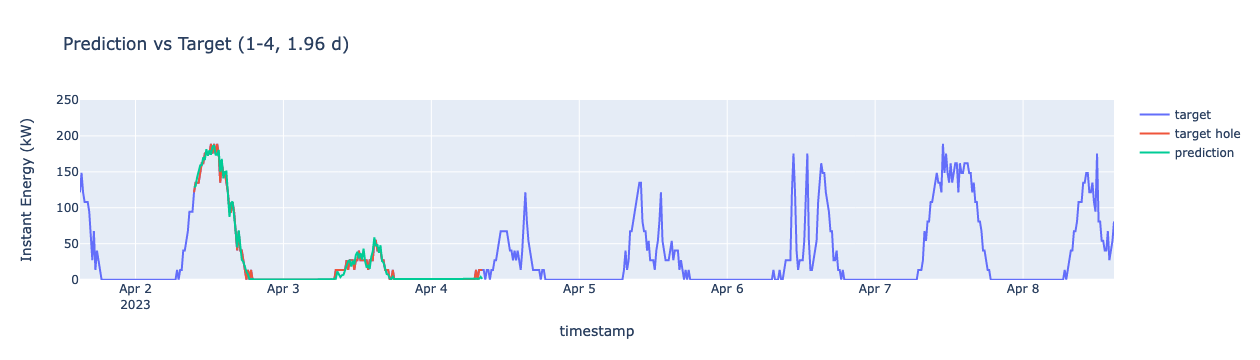
\includegraphics[width=\textwidth]{chapters/3_models/imgs/gab/eval/gabplotall1.png}
		\caption{}
	\end{subfigure}
	\begin{subfigure}{\textwidth}
		\centering
		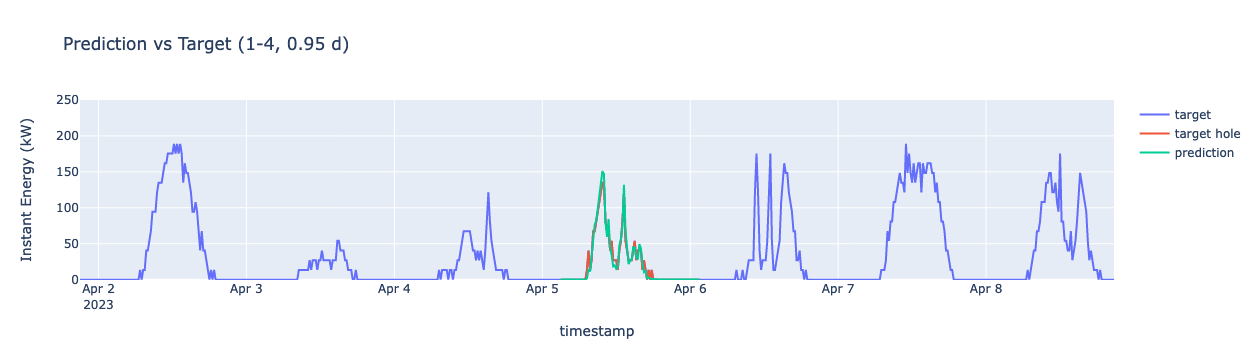
\includegraphics[width=\textwidth]{chapters/3_models/imgs/gab/eval/gabplotall2.png}
		\caption{}
	\end{subfigure}
	\begin{subfigure}{\textwidth}
		\centering
		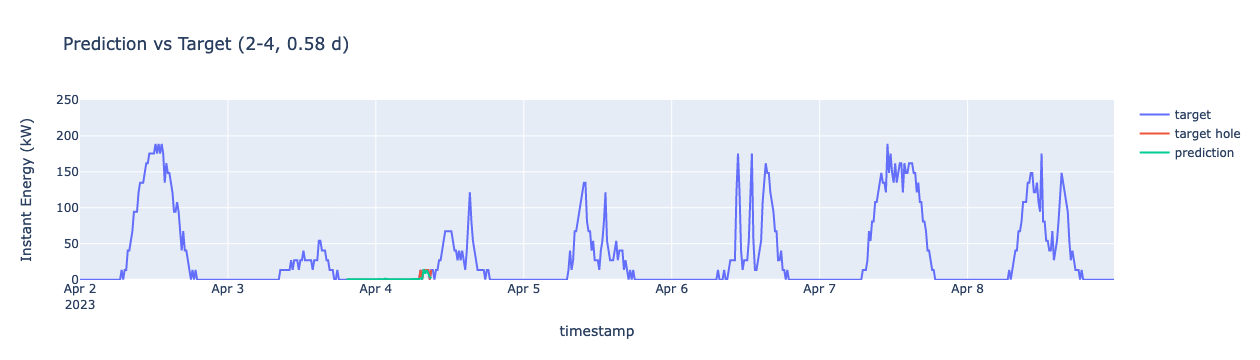
\includegraphics[width=\textwidth]{chapters/3_models/imgs/gab/eval/gabplotall3.png}
		\caption{}
	\end{subfigure}
	\caption{This figure shows some of the input time series provided to the model during the testing phase. We can see the entire series (in blue), the ground truth only for the gap period (in red), and the model's output only in the relevant gap period (in green). In graph (a), we have a gap size of almost two days, in (b) almost one day, and in (c) just over half a day.}
	%In questa Figura vengono mostrate alcune serie temporali passate in input al modello durante la fase di testing. Possiamo vedere l'intera serie (in blu), la ground truth solo del buco (in rosso) e l'output del modello solo nel periodo di buco interessato (in verde). Nel grafico (a) abbiamo una gap size di quasi due giorni, in (b) di quasi un giorno ed in (c) di poco più di metà giorno. }
	\label{fig:gaballplotsgaps}
\end{figure}


\begin{figure}[H]
	\centering
	\begin{subfigure}{\textwidth}
		\centering
		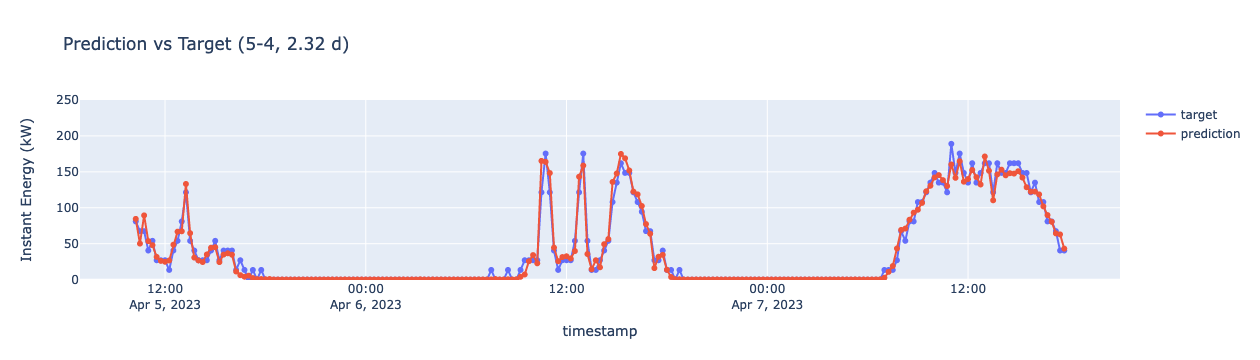
\includegraphics[width=.95\textwidth]{chapters/3_models/imgs/gab/eval/gabbuco5.png}
		\caption{}
	\end{subfigure}
	\begin{subfigure}{\textwidth}
		\centering
		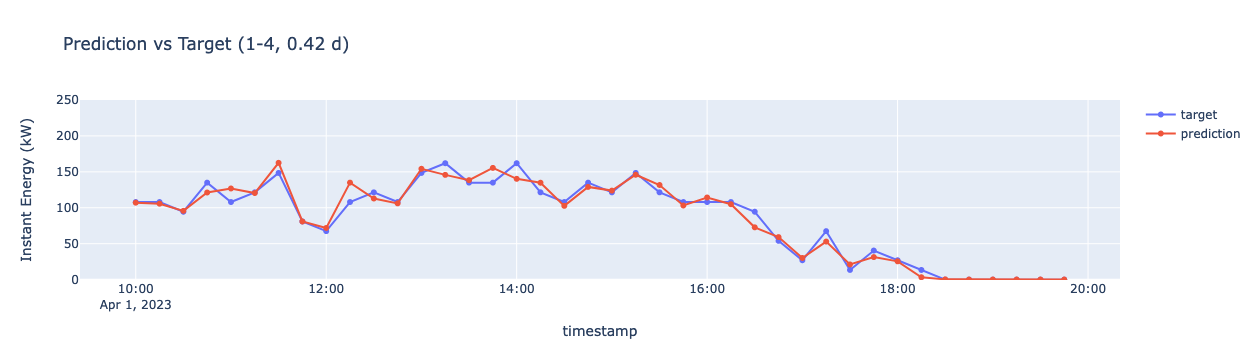
\includegraphics[width=.95\textwidth]{chapters/3_models/imgs/gab/eval/gabbuco2.png}
		\caption{}
	\end{subfigure}
	\begin{subfigure}{\textwidth}
		\centering
		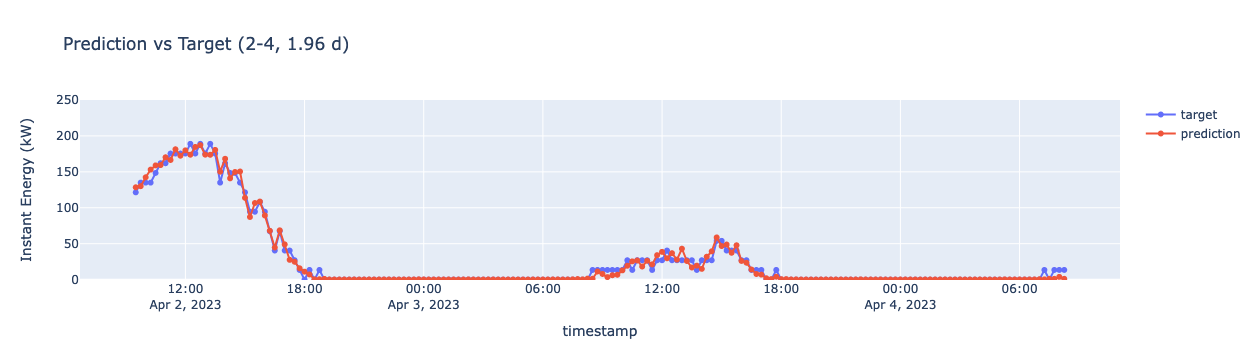
\includegraphics[width=.95\textwidth]{chapters/3_models/imgs/gab/eval/gabbuco3.png}
		\caption{}
	\end{subfigure}
	\begin{subfigure}{\textwidth}
		\centering
		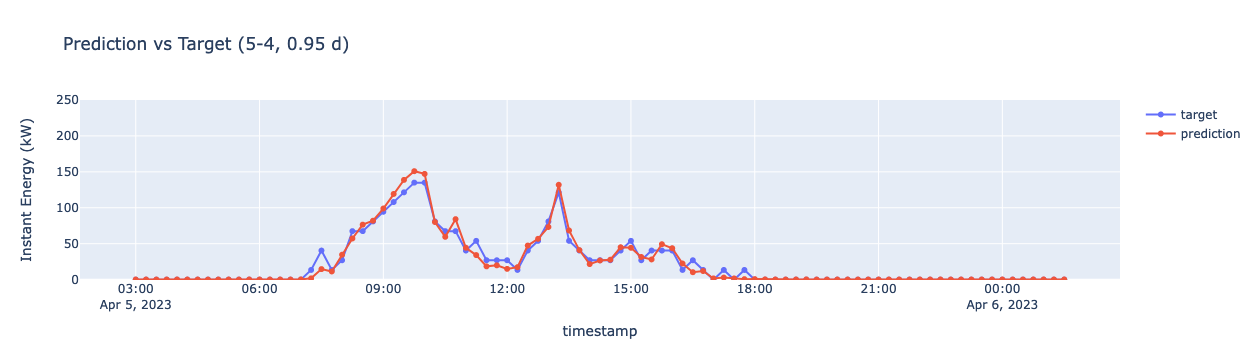
\includegraphics[width=.95\textwidth]{chapters/3_models/imgs/gab/eval/gabbuco4.png}
		\caption{}
	\end{subfigure}
	\caption{This figure displays some results of the model obtained during the testing phase, using gaps of varying lengths. You can see the model's outputs (in red) compared to their respective ground truths (in blue).}
	%Nella figura sono mostrati alcuni risultati del modello ottenuti durante la fase di testing, utilizzando gap size di lunghezza variabile. Possiamo vedere gli output del modello (in rosso) confrontati con le relative ground truth (in blu).}
	\label{fig:gabsolobuchi}
\end{figure}

Analyzing the results of the evaluation phase presented partly in Table~\ref{tab:gabpmaer} and in the graphs in Figure~\ref{fig:gabsolobuchi}, we can see that this model is very effective in predicting instantaneous energy during gaps of varying sizes. It excels in this task, whether for gaps of nearly a day or up to three days. We can observe that the $R^2$ index in these cases is consistently high, almost always hovering around the value of 0.97, with relatively low MAE and MAPE values.

Examining the global metrics reported in Table~\ref{tab:gabglobalmetrics} (a), we can confirm these findings. It shows an extremely low average MAE of 3.83 kW with a standard deviation of 1.40 kW, an average MAPE of 18.49\% with a standard deviation of 7.99\%, and an average $R^2$ value of 0.97 $\pm$ 0.05. This demonstrates how the model effectively approximates the ground truth with very low errors.

%Analizzando i risultati della fase di valutazione mostrati in 
%parte nella Tabella~\ref{tab:gabpmaer} e dai grafici in Figura~\ref{fig:gabsolobuchi} possiamo vedere come questo
%modello sia molto performante nel predirre l'energia istantanea durante
%buchi di differente dimensione. Si nota come riesce bene in
%questo compito sia su buchi di quasi un giorno fino ad arrivare
%anche a tre giorni. Possiamo vedere come l'indice $R^2$ in questi casi sia notevolmente
%alto, aggirandosi quasi sempre sul valore di 0.97 con anche
%valori di MAE e MAPE relativamente bassi.
%Analizzando le metriche globali riportate nella Tabella~\ref{tab:gabglobalmetrics} (a) possiamo confermare queste affermazioni.
%Presenta un MAE medio estremamente contenuto di 3.83 kW con una 
%deviazione standard di 1.40 kW, un MAPE medio di 18.49\% con deviazione standard di 7.99\% ed un valore medio di 0.97$\pm 0.05$ per l'indice $R^2$.

%unrisulta estremamente
%variabile con una valor medio di 16.67\% e una deviazione standar di 25.26\%. Lo stesso si applica per l'indice $R^2$
%che presenta si un buon valore di 0.92 ma una deviazione
%standard decisamente elevata di 0.23.
%Queste performance non brillanti sono dovute dal fatto che
%il modello faccia fatica a individuare l'andamento di buhi
%con dimensioni estremamente ridotte come mostrato in Figura~\ref{} con le relative metriche riportate in Tabela~\ref{}.
%
%E' importante notare che il modello presenta alcune difficoltà
%nell'individuare il corretto valore del primo e dell'ultimo valore
%del buco. Difficoltà che non si presentano estremente di frequente
%e che non comportano gravi ripercussioni sulle performance di questo.
%
%L'architettura presenta però problemi nel gestire buchi di
%piccole dimensioni, non superiori ai 90 timestamp (che rappresentano quasi un giorno intero). In questi casi possiamo anche raggiungere
%valori di 0.60 per l'indice $R^2$ ed anche un errore medio del 40\%.
%
%\begin{figure}[H]
%    \centering
%    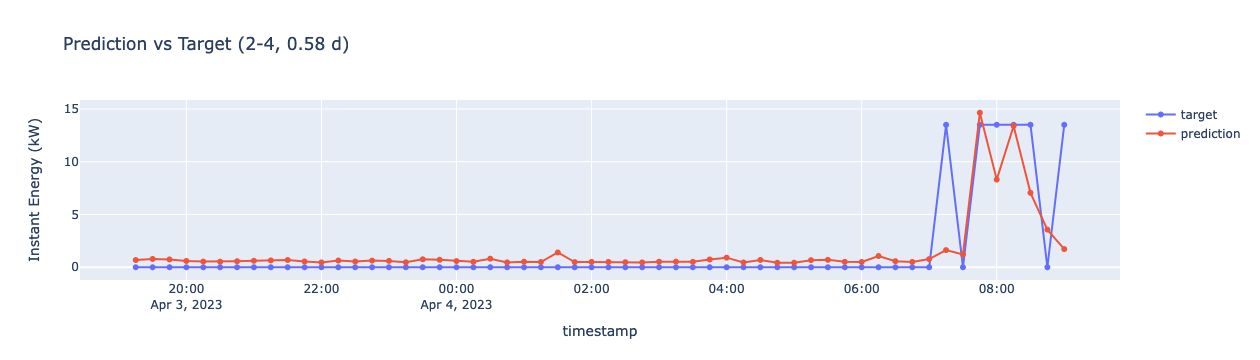
\includegraphics[width=\textwidth]{chapters/3_models/imgs/gab/eval/gabbucobrutto.png}
%    \caption{Nella figura viene mostrato un esempio di buco di piccole dimensioni dove il modello riscontra problemi nella predizione dell'energia istantanea. In questo caso abbiamo un MAE di 1.26 kW, un valore di 0.61 per l'indice $R^2$ e un MAPE del 45\%.}
%    \label{fig:enter-label}
%\end{figure}

\begin{figure}[H]
	\centering
	\begin{subfigure}{\textwidth}
		\centering
		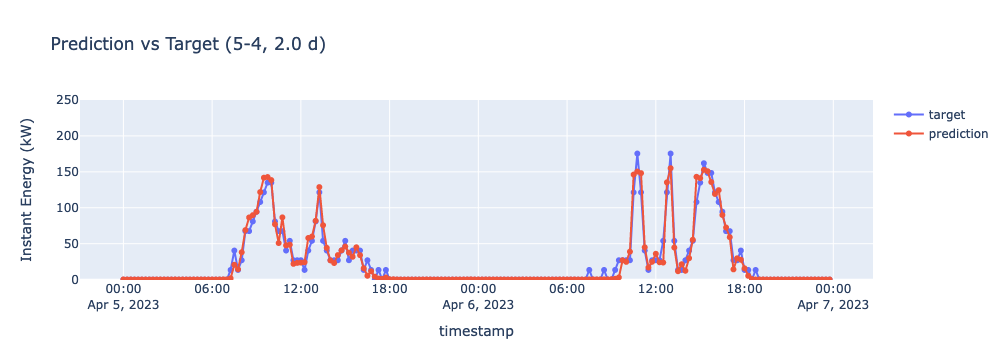
\includegraphics[width=\textwidth]{chapters/3_models/imgs/gab/eval/2days/gab2gionri54.png}
		\caption{}
	\end{subfigure}
	% \begin{subfigure}{\textwidth}
	%     \centering    
	%     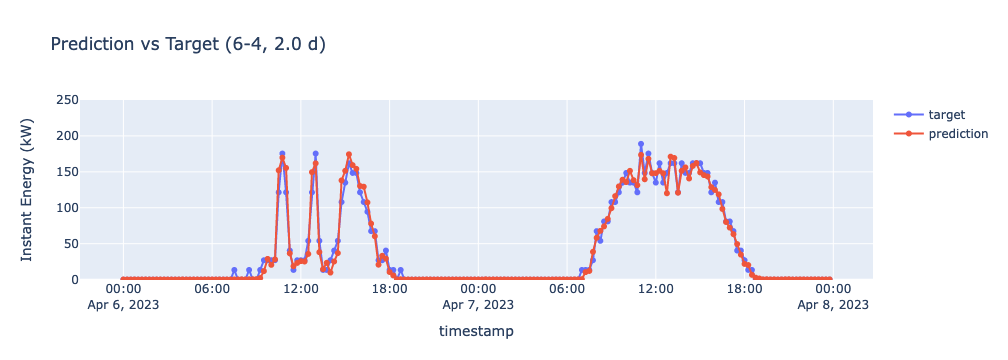
\includegraphics[width=.7\textwidth]{chapters/3_models/imgs/gab/eval/2days/gab2giorni64.png}
	%     \caption{}
	% \end{subfigure}
	\begin{subfigure}{\textwidth}
		\centering
		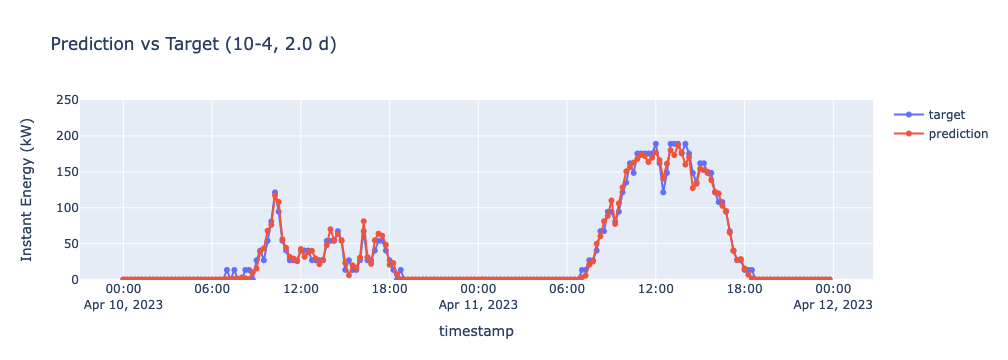
\includegraphics[width=\textwidth]{chapters/3_models/imgs/gab/eval/2days/gab2giorni104.png}
		\caption{}
	\end{subfigure}
	\caption{In this figure, some outputs from the testing phase of the model with a fixed 2-day gap size are presented. The model's predictions are shown in red, while the ground truth is in blue.}
	%Nella figura sono riportati alcuni output della fasi di testing del modello con gap size fissa a 2 giorni. Le predizioni del modello sono mostrate in rosso mentre la ground turth in blu.}
	%\caption{This figure displays some results of the model obtained during the testing phase, using gaps of varying lengths. You can see the model's outputs (in red) compared to their respective ground truths (in blue).}
	%Nella figura sono mostrati alcuni risultati del modello ottenuti durante la fase di testing, utilizzando gap size di lunghezza variabile. Possiamo vedere gli output del modello (in rosso) confrontati con le relative ground truth (in blu).}
	\label{fig:gabsolobuchi2giorni}
\end{figure}
\newpage
By repeating the evaluation phase with fixed gap sizes of two days to allow for a comparison with the other models, we can notice a slight improvement in the model's performance. Analyzing the data presented in Table~\ref{tab:gabglobalmetrics} (b), we have an average MAE of 3.76 $\pm$ 0.39 kW (2\% improvement with a 72\% better standard deviation), an average MAPE of 18.14 $\pm$ 6.76\% (2\% improvement with a 15\% better standard deviation), and an average $R^2$ value of 0.98 $\pm$ 0.02 (1\% improvement). In general, there is a 2\% overall increase in performance with a significant reduction in the standard deviation values.

%Ripetendo nuovamente la fase di valutazione e fissando a due giorni 
%le dimensioni dei buchi generabili, per permettere poi un confronto
%con gli altri modelli, possiamo notare un leggero incremento nell performance
%del modello. Analizzando i dai riportati in Tabella~\ref{tab:gabglobalmetrics} (b) abbiamo un
%MAE medio di 3.76$\pm 0.39$ kW (migliore del 2\% con deviazione standard migliore del 72\%), un MAPE medio di 18.14$\pm 6.76$ \% (migliore del 2\% con deviazione standard
%migliore del 15\%) ed un valor medio per l'indice $R^2$ di
%0.98$\pm 0.02$ (migliore del dell'1\%). In generale possiamo
%riscontrare un aumento delle performance generale del 2\%
%con un notevole abbassamento del valore delle deviazioni 
%standard.

\begin{table}[H]
	\begin{center}
		\begin{tabular}[c]{l|l|l|l}
			%\cline{2-4}
			\multicolumn{1}{c|}{\textbf{Gap Period}} &
			\multicolumn{1}{c|}{\textbf{MAE (kW)}}   &
			\multicolumn{1}{c|}{\textbf{MAPE (\%)}}  &                     % * 100
			\multicolumn{1}{c}{\textbf{R}$^2$}                             \\
			\hline

			04-04 to 05-04                           & 3.72 & 30.48 & 0.96 \\
			05-04 to 06-04                           & 4.25 & 26.99 & 0.96 \\
			06-04 to 07-04                           & 4.59 & 20.39 & 0.98 \\
			07-04 to 08-04                           & 4.33 & 15.29 & 0.98 \\
			08-04 to 09-04                           & 3.72 & 22.86 & 0.97 \\
			09-04 to 10-04                           & 3.52 & 29.76 & 0.94 \\
			10-04 to 11-04                           & 3.88 & 20.91 & 0.99

			% 06-04 to 07-04 & 20.07 & 0.62 &1293.53&50.70&1293.53&25.22 \\
		\end{tabular}
	\end{center}
	\caption{The table displays the values of MAE (Mean Absolute Error), MAPE (Mean Absolute Percentage Error), and the R$^2$ (R-squared) index applied to some model predictions made during the testing phase with a fixed gap size of 2 days. Some of these predictions are shown in Figures~\ref{fig:gabsolobuchi2giorni}.}
	%\label{tab:gabpmaer}
	%La tabella mostra i valori del MAE e dell'indice R$^2$ applicate alle predizioni del modello mostrate nelle Figure~\ref{fig:ufcnevalbelli} e \ref{fig:ufcnevalbrutti}.}\label{tab:dfsplit}
\end{table}

In conclusion, we can affirm that, despite the more demanding training phase, this model excels in the task of estimating instant energy production during periods of significantly variable gap sizes, achieving significantly better MAE, MAPE, and R$^2$ index values compared to those of the previous architectures.

%In conclusione possiamo affermare che, nonostante la più impegnativa fase di training, questo modello eccelle
%nel compito di stimare l'energia istantanea prodotta durante periodi
%di buchi con dimensione notevolmente variabile, riscontrando valori di MAE, MAPE e indice $R^2$ nettamente migliori rispetto a quelli delle precedenti architetture.
%

%\begin{table}[H]
%    \centering
%    \begin{tabular}{l|l|l|l|l}
%    \multicolumn{1}{c|}{\textbf{Gap}} &
%    \multicolumn{2}{c|}{\textbf{SAE (kW)}} &
%    \multicolumn{2}{c}{\textbf{SAPE (\%)}} \\
%    \hline
%    & Day 1 & Day 2 & Day 1 & Day 2\\
%    \hline
%
%    03-04 to 04-04 & 44.40 & 44.40 & 4.98 & 03.04\\
%    04-04 to 05-04 & 02.51 & 02.51 & 0.17 & 00.11\\
%    05-04 to 06-04 & 79.61 & 79.61 & 3.78 & 03.12\\
%    06-04 to 07-04 & 39.49 & 39.49 & 1.54 & 00.76\\
%    07-04 to 08-04 & 71.99 & 71.99 & 1.40 & 02.02\\
%    08-04 to 09-04 & 139.91 & 139.91 & 3.94 & 10.16\\
%    09-04 to 10-04 & 37.49 & 37.49 & 2.72 & 02.27
%    \end{tabular}
%    \caption{Nella tabella vengono riportati i risultati della fase di valutazione con gap size fissa a due giorni.}
%    \label{tab:gabdailyerrori}
%\end{table}

% DEV STANDARD